% Metódy inžinierskej práce

\documentclass[10pt,twoside,slovak,a4paper]{article}

\usepackage[slovak]{babel}
%\usepackage[T1]{fontenc}
\usepackage[IL2]{fontenc} % lepšia sadzba písmena Ľ než v T1
\usepackage[utf8]{inputenc}
\usepackage{graphicx}
\usepackage{url} % príkaz \url na formátovanie URL
\usepackage{hyperref} % odkazy v texte budú aktívne (pri niektorých triedach dokumentov spôsobuje posun textu)

\usepackage{cite}
%\usepackage{times}


\title{Vývoj mobilných aplikácií modelom MDE\thanks{Semestrálny projekt v predmete Metódy inžinierskej práce, ak. rok 2021/22, vedenie: Ing. Vladimír Mlynarovič, PhD.}} % meno a priezvisko vyučujúceho na cvičeniach

\author{Oliver Hofer\\[2pt]
	{\small Slovenská technická univerzita v Bratislave}\\
	{\small Fakulta informatiky a informačných technológií}\\
	{\small \texttt{xhofer@stuba.sk}}
	}

\date{\small 14.december  2021} % upravte



\begin{document}

\maketitle

\begin{abstract}
Cieľom článku bude zamerať sa na vývoj mobilných aplikácií s použitím MDE (Model driven approach). Pri modelovom softvérovom programovaní sa konkrétne zameriam na využite UML na vytváranie diagramov. Tiež by som chcel popísať výhody a nevýhody tohto postupu. Následne si opíšeme rôzne typy diagramov UML, ktoré pri vývoji aplikácií môžeme využívať a následne si ich taktiež porovnáme. V ďalšej časti si popíšeme hlavnú výhodu tejto metódy, čo je generovanie kódu na základe vytvorených diagramov za použitia nástroja GenCode. Na koniec článku v časti ~\ref{zaver},si tento model zhodnotíme a urobíme záver.
\end{abstract}
\paragraph{Kľúčové slová:} Modelovanie, Vývoj mobilných aplikácií, MDE, Model driven engineering, Android, UML


\section{Úvod}

Smartfóny so v dnešnej dobe súčasťou nášho každodenného života. Tieto malé zariadenia často nahrádzajú veľké stolové počítače alebo notebooky. Ešte pred pár rokmi by sme to o týchto zariadeniach povedať nemohli. Zato môžeme ďakovať hlavne vývoju hardvéru a softvéru. \newline
Taktiež za to môžeme ďakovať MDE (Model driven engineering), ktoré veľmi pomáha zefektívňovať písanie kódu. Ako tento spôsob funguje sa dozviete ďalej v článku v časti~\ref{MDE spôsob pre Android}.\newline
Momentálne väčšina zariadení používa systém Android, a preto som sa aj rozhodol sa zamerať v tomto článku konkrétne na tento systém.

\newpage
\section{Myšlienková mapa} \label{Myšlienková mapa}


\begin{center}
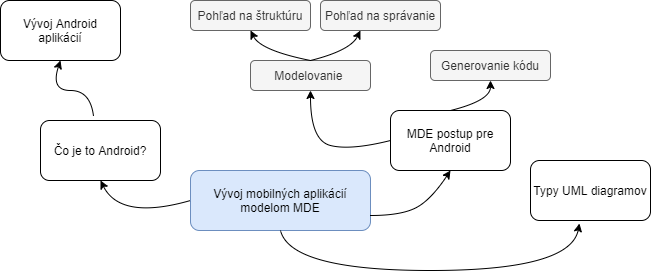
\includegraphics[scale=0.51]{myšlienková mapa.png}
Obr. 1: Myšlienková mapa.
\end{center}
V myšlienkovej mape môžeme vidieť časti, ktorým sa plánujeme v článku venovať. Ako prvé si povieme čo je to Android v časti ~\ref{Čo je to Android?}. Následne na to nadviažeme a povieme si ako sa tieto aplikácie vyvíjajú v časti ~\ref{Vývoj Android aplikácii}. 
Potom si pri bode MDE postup pre Android v časti ~\ref{MDE spôsob pre Android} povieme niečo bližšie o modelovaní a generovaní kódu. Modelovanie si ďalej rozdelíme na pohľad na štruktúru a pohľad na správanie. Nakoniec si bližšie popíšeme UML diagramy použité pri vytváraní Android aplikácii v časti ~\ref{Typy UML diagramov}.


\section{Čo je to Android?} \label{Čo je to Android?}
Android je rozsiahla open-source platforma založená jadre Linuxu. Tento operačný systém je vlastnený spoločnosťou Google. \cite{Android1}Tento systém bol pôvodne vytvorený skupinou developerov známych ako Open Handset Alliance, ktorá bola sponzorovaná firmou Google. \newline
Tento systém sa začal vyvíjať v októbri 2003. Avšak pôvodne bol vytvorený pre digitálne fotoaparáty. Následne v roku 2005 túto firmu kúpila spoločnosť Google a začala ho používať ako operačný systém pre mobilné zariadenia. \cite{Android2}\newline
V dnešnej dobe sa však nepoužíva len v  Mobilných telefónoch. Používa sa aj v tabletoch, televíziách, nositeľných zariadeniach, v systémoch v autách a mnoho ďalších zariadeniach.



\section{Vývoj Android aplikácii } \label{Vývoj Android aplikácii}

Android aplikácie boli v minulosti aj dnes vyvíjané za pomoci jazyku Java. Avšak dnes sa začínajú využívať alternatívy ako je Kotlin alebo Dart a mnoho ďalších. Pri písaní programu sa používajú SDK (Software development kit) čo je softvér nástrojov pre vývojárov. IDE (integrated Development Environment) čo je skratka pre integrované vývojové prostredie. \newline
Hlavné vývojové prostredie pre Android aplikácie je Android Studio, ktoré poskytuje flexibilnú platformu pre developerov, kde môžu používať rôzne SDK. Pre jazyky Kotlin a Java sa používa rovnaké SDK ale jazyk Dart používa SDK, ktoré sa volá Flutter. \newline
Súčasťou SDK je väčšinou Dalvik. Dalvik je virtuálny stroj na, ktorom beží operačný systém Android. Využíva sa na rýchle testovanie aplikácií bez potreby pripájať mobilné zariadenie. Tento nástroj tiež veľmi zefektívňuje proces programovanie.\newline
Hlavnou zložkou Android aplikácií je Aktivita. Android aplikácia väčšinou obsahuje jednu alebo viac aktivít. Aktivita sa zobrazuje ako jedno používateľské prostredie, ktoré si vieme predstaviť ako karty s prvkami, s ktorými môže užívateľ pracovať.\newline
Servis je špeciálna aktivita, ktorá nemá užívateľské rozhranie a pracuje na pozadí. Pracujú na aplikačnej rámcovej vrstve (App Framework Layer). Spolu s aktivitou sú to najpoužívanejšie komponenty pri programovaní Android Aplikácií. \newline
Každá aktivita v Android kóde má svoj životný cyklus (lifecycle). Je to vlastnosť aplikácie, ktorá určuje čo sa má s určitou aktivitou diať v určitých prípadoch. Napríklad, čo sa stane s aktivitou keď sa spustí aplikácia alebo čo sa stane s aktivitou keď sa aplikácia stane... \cite{VývojAndroid}








\section{MDE postup pre Android} \label{MDE spôsob pre Android}

\subsection{Modelovanie}\label{MDE spôsob pre Android:Modelovanie}
Tento spôsob popisuje ako kompletne popísať štruktúru a správanie Android aplikácie použitím štandardu UML. \newline
Pri tomto postupe sú aplikácie modelované za pomoci UML diagramov tried, ktoré sa využívajú na vytvorenie pohľadu na štruktúru, o ktorej si povieme v časti ~\ref{MDE spôsob pre Android:Modelovanie:Pohľad na štuktúru}. A za pomoci diagramov postupnosti vieme generovať kód správania nášho programu, o pohľade na správanie si povieme viac v časti ~\ref{MDE spôsob pre Android:Modelovanie:Pohľad na správanie}. \cite{GenerovanieAndroid}

\subsubsection{Pohľad na štuktúru}\label{MDE spôsob pre Android:Modelovanie:Pohľad na štuktúru}
Z diagramov tried generujeme štrukturálny kód. Pri pohľade na štruktúru sa ako programátori pozeráme na dva základné komponenty,  aktivity a servisy. Sú to špeciálne komponenty, ktoré sa používajú na definovanie základnej aplikačnej štruktúry. V tejto štruktúre by malo byť bližšie špecifikované, ktoré triedy sú aktivity a servisy. Na nasledujúcom obrázku môžeme vidieť znázornenie, kde je Main (Hlavná časť kódu) definovaná ako Aktivita a Pozadie definovaná ako Servis. \newline
Vyššie spomenuté komponenty môžu nadobúdať určité metódy o ktorých sme si už hovorili v části ~\ref{Vývoj Android aplikácii}. Tieto metódy môžu byť volené programátorom.\newline
Tiež z diagramov tried program vie vygenerovať atribúty funkcií a vlastnosti objektov.\cite{GenerovanieAndroid}\cite{GenerovanieJava}
\begin{center}
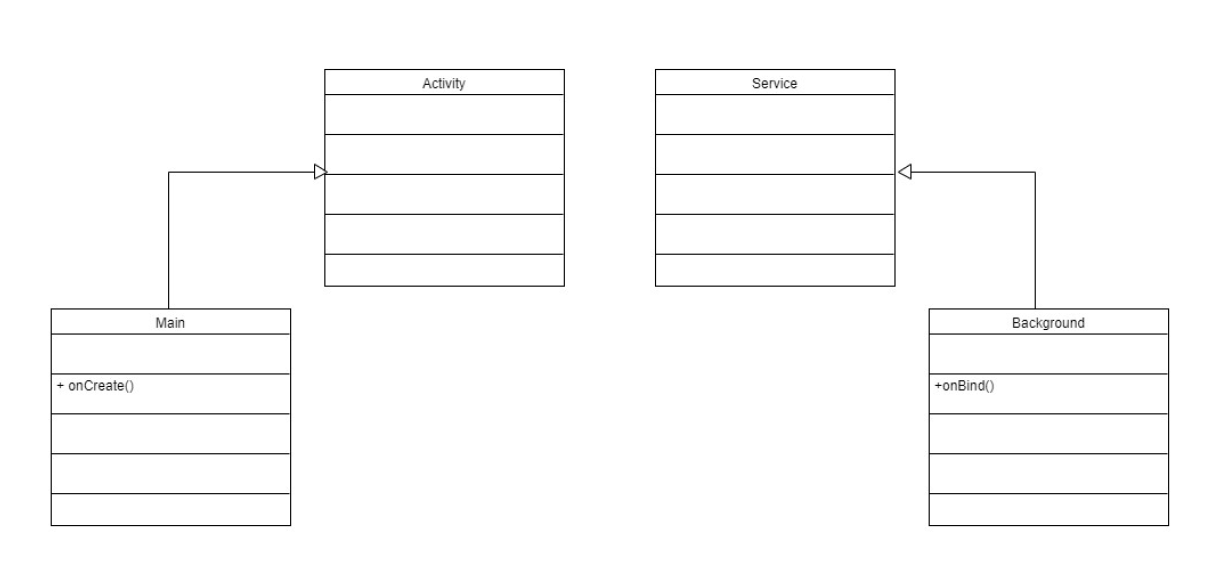
\includegraphics[scale=0.5]{diagram.png}
Obr. 2: Myšlienková mapa, upravené podľa:\cite{GenerovanieAndroid}
\end{center}

\subsubsection{Pohľad na správanie}\label{MDE spôsob pre Android:Modelovanie:Pohľad na správanie}
Ako sme už vyššie spomínali, pri pohľade na správanie používame diagramy postupnosti. Tieto diagramy vedia znázorňovať rôzne podmienky, cykly, iterácie, atď. Bohužiaľ má to aj svoje chyby. Nie všetky časti kódu sa dajú vygenerovať. Bližšie si o tom povieme v nasledujúcej časti ~\ref{Generovanie kódu}.\cite{GenerovanieAndroid} \cite{GenerovanieJava}

\subsection{Generovanie kódu}\label{Generovanie kódu}
Hlavným benefitom adaptovania MDE postupu pri vyvíjaní Android aplikácii je automatizácia v podobe generovania kódu. Na generovanie kódu môžeme použiť diagramy tried alebo diagramy postupnosti.\newline
Z diagramu tried program na generovanie vygeneruje základnú aplikačnú štruktúru a súbory v jazyku Java pre každú triedu. Obsahuje definície tried a atribúty funkcií. Tiež obsahuje konštruktor a metódy. Z tohto diagramu si vie aplikácia GenCode vie zistiť vzťahy medzi triedami. Keď trieda obsahuje API, program do nášho kódu zahrnie potrebné balíky pre chod programu.\newline
Bohužiaľ generovanie kódu na základe grafov postupnosti má svoje limity. Napríklad jednoduché operácie ako generovanie dynamicky alokovaných polí nesú možné. Avšak dokáže generovať časti kódu ako podmienky a cykly.\cite{GenerovanieAndroid}



\section{Typy UML diagramov} \label{Typy UML diagramov}
    \subsection{Diagramy tried}\label{Typy UML diagramov:Diagramy správania}
    Tento typ diagramu je jeden z najviac populárnych diagramov medzi softvérovými inžiniermi. Je to typ diagramu štruktúr. Jednotlivé komponenty takého diagramu reprezentujú triedy, objekty alebo vzťahy medzi triedami a objektami.\newline
    Tvar triedy pozostáva z obdĺžnika s tromi riadkami. Prvý riadok obsahuje názov triedy, druhý riadok atribúty a tretí riadok obsahuje metódy triedy ktoré používame. \cite{DiagramyTried}

    \subsection{Diagramy správania}\label{Typy UML diagramov:Diagramy štruktúry}
    Diagramy správania (Diagramy postupnosti) sa dá v skratke nazvať ako diagram vzťahov. Diagram vzťahov preto, lebo popisuje ako a v akej postupnosti spolu objekty pracujú.\newline
    Tieto diagramy používajú softvérový developeri a profesionáli v oblasti obchodu, aby pochopili požiadavky nového systému alebo na zdokumentovanie existujúceho procesu. \cite{DiagramySprávania}

\section{Reakcie na prednášky} \label{Reakcie na prednášky}

 \paragraph{Spoločenské súvislosti.}Podľa môjho osobného názoru prednáška s dekanom našej fakulty bola veľmi zaujímavá. Bolo zaujímavé počúvať o tom ako práca v IT vplýva na nás a na naše okolie. \newline
Taktiež som si uvedomil, aký je tento sektor dôležitý hlavne v aktuálnej pandemickej situácii. Práca z domu je čoraz bežnejšia a mobilné aplikácie používame na dennej báze. Používame ich napríklad na komunikáciu s inými ľuďmi. Tieto mobilne aplikácie nám umožňujú spájať sa s kolegami, učiteľmi aj bez nutnosti byť v škole alebo práci.\newline
Tiež som si uvedomil aké je v dnešnej dobe dôležité vzdelanie. Obzvlášť dôležité je v IT sfére kde si niektoré firmy vyžadujú vysokoškolské vzdelanie alebo zamestnanci s vysokým vzdelaním sú lepšie ohodnotený.

 
 \paragraph{Historické súvislosti.}Táto prednáška bola taktiež veľmi zaujímavá a náučná. Bola o osobnostiach informatiky, ktorí významne do tohto odvetvia prispeli svojimi vedomosťami. Niekedy si ani neuvedomujeme aké to muselo byť náročne niečo také vyvinúť v dobe, v akej sa nachádzali. V dobe, kedy nebolo prístupných toľko informácií akom máme teraz dostupných na internete. V dobe, kedy nemali k dispozícii techniku, ktorá nám v dnešnej dobe zjednodušuje život. Aj napriek tomu boli schopný vymyslieť neuveriteľné zariadenia alebo funkcie. \newline
 Ale doba ide dopredu. V dnešnej dobe je mnoho vynálezov, ktoré nám zefektívňujú našu robotu. Ako napríklad generovanie kódu na základe UML diagramov čo vie zjavne urýchliť vývoj nových mobilných aplikácií.
 
 \paragraph{Technológia a ľudia.}Prednáška na túto tému sa mi osobne páčila. Bola zaujímavá a náučná ako všetky prednášky v tomto semestri. \newline
Technológie sú medzi nami už od pradávna. Od prvých vynálezov ich hlavným cieľom bolo, zjednodušovať si každodenné úlohy. Iné to nie je ani v dnešnej dobe. Pri programovaní používame množstvo technológií, ktoré nám tento proces zefektívňujú. Preto som si vybral aj túto tému, v ktorej hovorím o možnosti generovania kódu z UML diagramov. 


 
 

\section{Záver} \label{zaver} % prípadne iný variant názvu
V tomto článku sme si ukázali, ako môžeme použiť modelovanie pri tvorbe Android aplikácii. Modelovanie sme konkrétne využili pri generovaní kódu za pomoci UML diagramov. Tento postup má veľa výhod. Najhlavnejšia výhoda je určite rýchlosť písania kódu. Avšak sú tam aj nevýhody, o ktorých sme si povedali v časti .\newline
Podľa môjho názoru je táto téma veľmi zaujímavá a má veľkú perspektívu do budúcnosti. 



%\acknowledgement{Ak niekomu chcete poďakovať\ldots}


% týmto sa generuje zoznam literatúry z obsahu súboru literatura.bib podľa toho, na čo sa v článku odkazujete
\bibliography{literatura}
\bibliographystyle{unsrt} % prípadne alpha, abbrv alebo hociktorý iný
\end{document}
